\documentclass[12pt, a4paper]{article}
\usepackage[margin=1in]{geometry}
\usepackage{tikz}
\usepackage{graphics}
\usepackage{amsmath}
\usepackage{amssymb}
\usepackage{subfig}

% Title Page
\title{Evolving Tower-Destroying Robots:\\\normalsize An Exploration into Scaffolded Learning}
\author{Ryan Boldi}


\begin{document}
\maketitle
\tableofcontents

\newpage
\section{Goals}
We do not teach linear algebra to 6 year olds due to the fact that they do not have sufficient educational \emph{scaffolding} to grasp such a bizarre concept. My goal was to see whether or not this also applies to a robot evolving to do a certain task.\par 
The robot's task is to destroy a tower that starts a specific distance away from it:\par
\vspace{-10pt}
\begin{figure}[h]
	
\begin{center}
	\centering
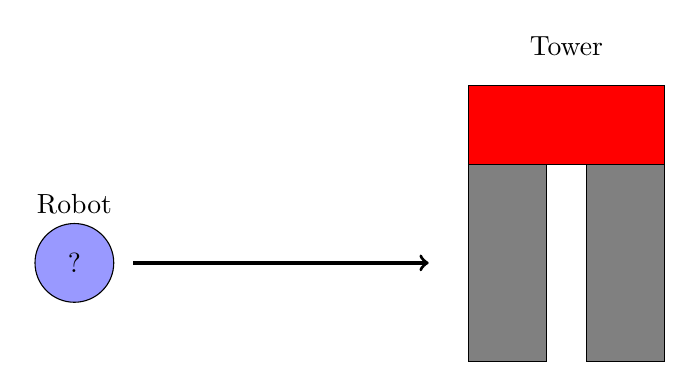
\begin{tikzpicture}
\filldraw[fill=blue!40!white](0,1.25) circle (5mm);
\node[] at (0,1.25) {?};
\node[] at (0,2) {Robot};
\draw [->, very thick] (0.75, 1.25) -- (4.5,1.25);
\filldraw[fill=gray] (5,0) rectangle (6,2.5);
\filldraw[fill=gray](6.5,0) rectangle (7.5,2.5);
\filldraw[fill=red] (5,2.5) rectangle (7.5,3.5);
\node[] at (6.25,4) {Tower};
\end{tikzpicture}
\caption{Diagram demonstrating the robot's task.}
\label{goal}
\end{center}
\end{figure}
\vspace{-10pt}
To scaffold the learning of the robot, I planned to start the tower close to the robot, and slowly move it farther and farther away over the course of many generations. This will continue until the tower is at the goal distance from the robot. These are environmental changes that starts the robot with an easy task, waits for the task to be completed, then makes the task slightly harder. This process is repeated until the robot has mastered the most difficult goal task.\par
My goal was to experiment with this process, seeing whether or not it actually improved the speed of solution discovery, or quality of the solutions themselves.
\newpage

\section{Implementation}
\paragraph{Robot}
I started by creating the robot. It was based on a simple quadruped, but with 2 added arms to make destroying the tower easier. All of the limb relative sizes can be controlled and fined tuned in \emph{constants.py}.\par
\begin{figure}[h]
	\centering
	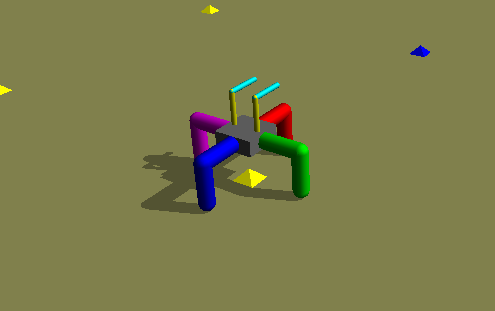
\includegraphics{robot.png}
	\caption{The \emph{Tower-Destroyer} Robot. It has 6 sensors: one on the tip of each limb. It may move its legs and arms freely, each with 2 degrees of freedom. Each motor is controlled by the output layer of a fully connected neural network, which takes the sensor data as inputs. }
\end{figure}
\paragraph{Tower}
The tower is created out of 3 similar cuboids, with the third balanced on top of the bottom two (see figure~\ref{goal}). The block colored in red is to be my `fall detector'. If this block drops below a certain $y$-level, we will count this tower as ``fallen". If the tower has fallen over, the robot will receive a large fitness reward.
\paragraph{Fitness} To ensure that the reinforcement is not too sparse, I wanted to include an incentive to move towards the tower. After much deliberation, this is the fitness function I have included:
$$
\text{Fitness} = \begin{cases}
\text{distance from origin}_y & \text{if tower did not fall};\\
20 & \text{if tower fell.}\\
\end{cases}
$$

\noindent I believed that this would promote movement in the positive $y$ direction before the tower is in the robot's reach.

\paragraph{Scaffolding} To control whether or not we are going to scaffold the robot's learning, I added a new constant to the program that controls how many generations of \emph{pretraining} will occur. During pretraining, the tower's distance starts at low value, and incrementally gets larger as the robot performs better. When these pretraining generations are completed, the tower's distance will be set to the maximum (goal) distance, and the evolution continues until all of the total generations have completed. If pretraining is set to 300, and total generations is set to 600, we will pretrain the population for 300 generations, slowly incrementing the tower's distance whenever a robot successfully knocks over the tower. At 300 generations, no matter the current distance of the tower, we move it to it's maximum distance for the final 300 generations. If pretraining is set to 0, and total generations is set to 600, we will start the tower at its maximum distance, and train the population on that for 600 generation without moving the tower.
\newpage
\section{Results}
I expected to see the robots that were pretrained in the simpler environment doing better than robots that were solely trained on the difficult environment. If this was the case, we would see the robots that have been pretrained for half of the total evolutionary time do better in that second half where they are in the difficult environment than a robot trained on the difficult environment for all the generations. This provides us with a fair means of comparison between the two evolutionary methods. 
\begin{figure}[h]
	\centering
	\title{No Pretrain, 600 Total}
	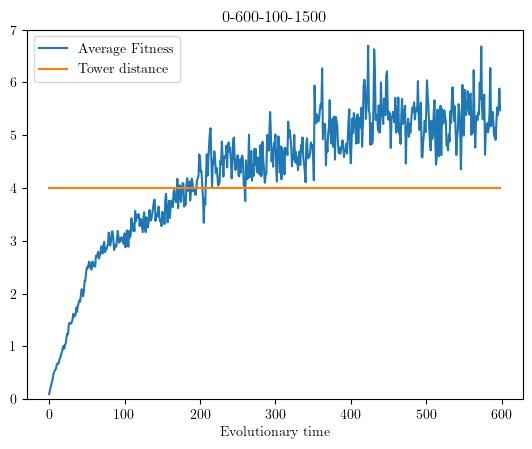
\includegraphics[width=1\textwidth]{0-600-100-1500/0-600-100-1500.png}
	\caption{Result after 100 robots were evaluated for 1500 timesteps per generation over the course of 600 generations, 0 of which are pretraining. Because there was no pretraining, the tower stays at a constant distance away from the robot over the entire course of evolution. The fitness of the robots is their distance from the origin in the $y$ direction, so the point where the blue and orange lines meet effectively represents when the robots reach the tower. Past this, the only way to get fitness is to destroy the tower, which is how the fitness continues to increase.}
	\label{nopretrain}
\end{figure}

Figure~\ref{nopretrain} proves that evolution did in fact take place. We can see that the evolved creatures in generation 600 perform much better than the randomly evolved creatures in generation 0 (as they have a higher average fitness).

Next, I repeated evolution, but set pretrain to 300. This means that half of evolution will take place in the pretrain phase, where the tower gets incrementally farther away, until generation 300, where the tower is set to its maximum distance.

%discuss that this was what i expected, eventually, due to the fact that i give them inentive to move forward, the robots will learn to walk towards the tower, and one of them will eventually break down the tower.
%in the future, i could maybe vary where the tower is, so that the creatures that train on the closer towers have an easier time when it gets further away


\begin{figure}[h]
\title{300 Pretrain, 600 Total}
\centering
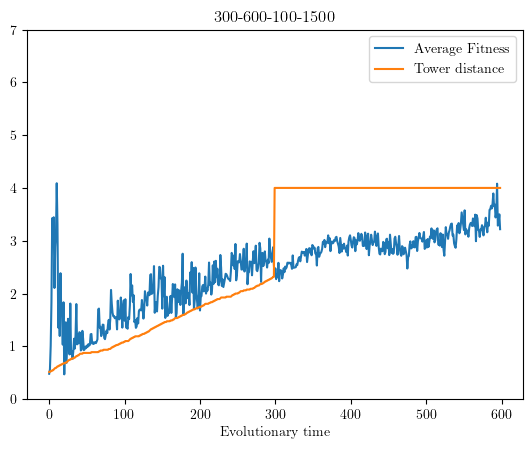
\includegraphics[width=1\textwidth]{300-600-100-1500/300-600-100-1500.png}
\caption{Result after 100 robots were evaluated for 1500 timesteps per generation over the course of 600 generations of evolution, 300 of which are pretraining. We can see that the robots are able to destroy the tower at the beginning, but as the tower gets farther away they are less able to do so. We can see that after 300 generations, none of the robots are able to knock over the tower as it is at its maximum offset of 4. There is a large spike of fitness at the beginning due to how easy it is to destroy the tower (just falling forward). Only in one of the last generations was a robot able to knock over the tower (because the blue line is above the orange line, therefore the average fitness is larger than the distance to the tower).}
\end{figure}

This result surprised me. It completely went against my hypothesis as the creatures that were pretrained in fact did \emph{worse} when the tower was 4 units away. I decided to change the population size and generation count, to see if, given more time, the pretrained population would eventually increase their fitness.
\begin{figure}[ht]
\centering
\subfloat[0 Pretrain, 1000 Total]{
	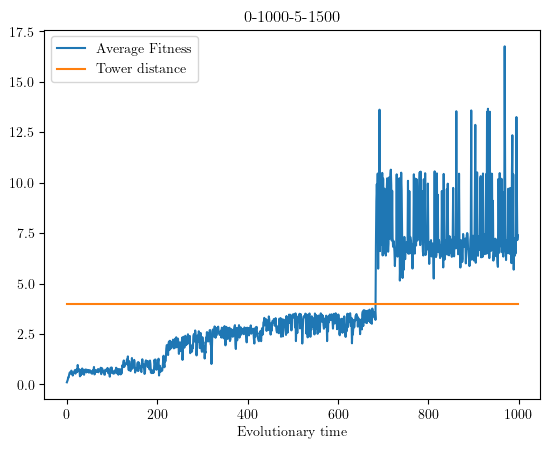
\includegraphics[width=0.45\textwidth]{0-1000-5-1500/0-1000-5-1500.png}
	\label{0-1000-5}
}
\quad
\subfloat[500 Pretrain, 1000 Total]{
	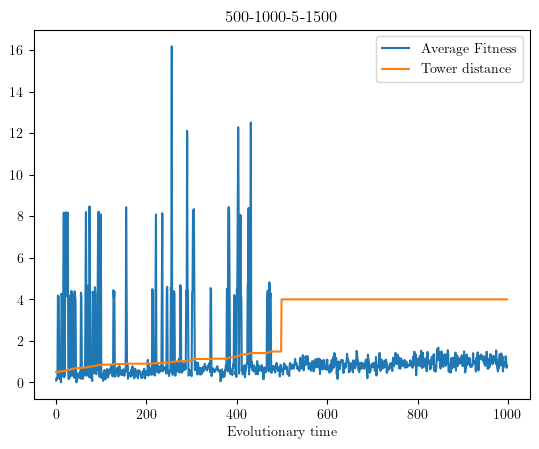
\includegraphics[width=0.45\textwidth]{500-1000-5-1500/500-1000-5-1500.png}
	\label{500-1000-5}
}
	\caption{Result after 5 robots were evaluated for 1500 timesteps per generation, over the course of 1000 generations of evolution.  Once again, the evolutionary run without pretraining managed to find a solution. We can see that the first robot destroys a tower at around generation 700 (for a population of 5 creatures, this is normal). Figure~\ref{500-1000-5} shows this same experiment \emph{with} pretraining.}
\end{figure}
Once again, the run with pretraining starts off easy (as seen by the abundant reward in the first 500 generations), but after the pretraining is up, the creatures have no chance adapting to the difficult environment, and stay relatively consistent in moving ${\thicksim}0.7$ units away from the origin in the $y$ direction. 

As we can see, the results are consistent with the earlier run. Figures~\ref{0-1000-5} and~\ref{500-1000-5} show that pretraining is adversely affecting evolution. We can tell that this is the case because the evolutionary run without pretraining yields a solution that can destroy the tower at its maximum distance of 4. Yet, with pretraining, the robots do not destroy the tower at all when it is at its maximum distance. As shown in figure~\ref{0-1000-5}, it took around 700 generations for a robot controller to be discovered that can destroy the tower. But, with pretraining, no robot comes close to destroying the tower for portion of evolution where the tower is at 4 units away.

To ensure that these results were not just coincidences, I ran evolution one final time, and gave the pretraining many more generations to help smoothen the transition from pretrianing to regular evolution.

\begin{figure}[ht]
\centering
\subfloat[0 Pretrain, 6000 Total]{
	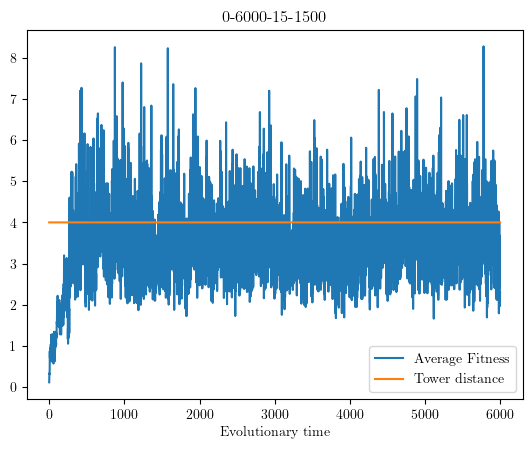
\includegraphics[width=0.45\textwidth]{0-6000-15-1500/0-6000-15-1500.png}
}	
\quad
\subfloat[3000 Pretrain, 6000 Total]{
	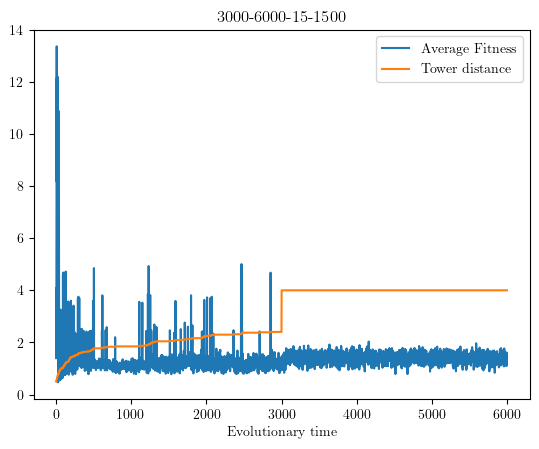
\includegraphics[width=0.45\textwidth]{3000-6000-15-1500/3000-6000-15-1500.png}	
}
\caption{Once again, the robots that were trained without any pretrain performed, on average, much better than the creatures that did pretrain. This futher proves that pretraining is adversely affecting the time it takes to come to a solution.}
\end{figure}

\newpage

\section{Reflection}
Through this experiment, I have learned that scaffolded learning does not always have a beneficial affect on the rate at which a solution is discovered by evolutionary algorithms. I will propose a couple of reasons as to why this might be the case.

\paragraph{Overfitting}
The first possible reason for this could be the robots overfitting to their environment, meaning they are not robust to changes in that environment. For example, when the robots first start with the tower 0.5 units away from them, a very effective strategy to destroy this tower would be to just learn forward and fall over onto the tower. Although this will provide vast amounts of fitness early on, when the tower gets farther away, this strategy becomes useless. This means the whole population will become offspring of that one ``fall forward" robot. Through this, we lose all the genetic diversity in our population, and the robots must re-evolve to move once the towers move farther away. Some robots that were pretrained discovered how to lean forward, fall, flip itself over, and walk on its hands to help move to the farther away towers. Although this does work, it is much less efficient to evolve, as well as a much slower gait.

\paragraph{Luck}
Although unlikely, it could be that these three experiments were not sufficient to comment on the patterns presented by this experiment, and I must repeat the experiment many more times to see if this is the case \emph{every} single time.

\subsection{Implementation Comments}
\paragraph{Difficulties} Implementing the robot body, robot neural network and tower was surprisingly easy. I expected to spend much longer trying to get everything to work as envisioned. However, figuring out when the tower fell over was surprisingly difficult. I could not just use a touch sensor on the top block, as this would always be triggered by the support blocks touching it. I ended up hacking together a simple checker that checks whether the top block's z value is less than half of what it started with. Further, saving and parsing the data took the most time, as I had to develop my own data saving and parsing system to automatically label the data with the evolutionary constants. I also had to manually change the settings in between runs.

\paragraph{Pyrosim} Pyrosim made this project very simple from a physics engine point of view. The only feature I would have liked to see would be a ball-in-socket joint to allow for 2 degrees of freedom in the robot's shoulders. I had to hack together a really crude ball in socket joint by putting a tiny cylinder in between the upper arm and the main body, with two orthogonal joints connecting them. 


\subsection{Future Work}
\paragraph{Queued experiments} If I had more time on this project, I would have developed a system to automatically do multiple evolutionary runs without human input. This would allow for very long training sessions without human dependency. I could set the program to test all 0,300,600,... generations, and save the data into the respective files.

\paragraph{Fitness Functions} I would like to change the way the fitness functions works as well. This is because the fitness function rewards forward locomotion even if the creature does not destroy the tower. This makes the tower not a necessary part of the experiment from a reward perspective, and it only becomes an obstacle for the creatures. I think that I would have changed the way fitness works to make the robot rely on destruction of the tower for reward.

\paragraph{Tower Movement} I could also move the tower around the world space. This might cause different results to appear. I think that part of the reason the creatures learned very quickly without any scaffolding was that the problem was very easy to solve. Walking in a straight line and knocking over the tower is not a very complex task (especially when the fitness function rewards it), so pretraining the robots would not even be needed to solve this problem. On the other hand, if the tower was not always directly infront of the robot, but slightly to the right or left, pretraining might come in handy in learning where the robot is located.

\paragraph{Task} In hindsight, the tower destruction task is not complex enough to require pretraining. This is because the tower ends up falling over if the robot just runs into it. To add value to pretraining, I would need to make the task something more specialized. For example, putting a ball in a  basket, pressing a button in an obscure location, or picking an obstacle up. These tasks are very difficult to learn on their own, so learning them at the same time as learning to walk would be difficult. Thus, pretraining might become useful in these experiments. 
\end{document}          
